\chapter{Overview of Rb magnetometer and apparatus}

%\begin{itemize}
%\item Purpose: Describe your experiment, focusing on the overall
%  function, and providing some description of the individual
%  components and their function.
%\item Outline:
%  \begin{itemize}
%  \item Overview of experimental apparatus.  I think this is done by
%    describing Figs.~\ref{fig:zerofield} and \ref{fig:pumpprobe}.
%  \item Group Fig.~\ref{fig:pumpprobe} into major components and
%    describe each one.  For example:
%    \begin{itemize}
%      \item ECDL and DAVLL
%      \item Pump beam and AOM
%      \item Probe beam and balanced polarimeter
%      \item Cell
%      \item Magnetic field system
%        \begin{itemize}
%        \item Shield arrangement
%        \item Degaussing system
%        \item Internal coil\underline{s}
%        \end{itemize}
%      \item DAQ
%    \end{itemize}
%  \item General operation is discussed in the next chapter.
%  \end{itemize}
%\end{itemize}

The purpose of this Chapter is to describe the experimental apparatus
used at UW.  The system is composed of three main parts:
\begin{itemize}
\item A tunable laser system, operating near the Rb D1 line.  Pump,
  probe, and laser characterization beams all come from this light
  source.  The beams are analyzed using various sensitive photodiode
  sensors.
\item A paraffin-coated natural Rb cell.  The cell provides a vapour
  pressure of Rb atoms whose spin state can remain coherent after many
  wall bounces.  The long coherence time is important for the best
  magnetometer sensitivity.
\item A magnetic shielding and field generation system.  The
  magnetometer is being operated in magnetic fields that are
  considerably smaller than Earth's field.  An aspect of the research
  also is to use the magnetometer to learn about magnetic field
  stability.
\end{itemize}
In this Chapter, I start with a more detailed overview of the overall
experiment.  I then discuss each of the major components of the
apparatus in more detail.

In Chapter~\ref{ch:characterization}, I will cover the initial
characterization of a few different modes of operation of the
magnetometer.  (As discussed in Chapter~\ref{ch:magnetometry}, there
are several different ways in which the magnetometer can be operated
dependent with different advantages and disadvantages to each.)

In Chapter~\ref{ch:results}, I discussed the advances made in the
understanding of the magnetometer performance, mostly in relation to
the development of the Free-Induction-Decay mode of operation.

%this section will be completed with the comparison of different
%possible operation modes of an atomic magnetometer and an introduction
%into the concepts of magnetometer uncertainties and the noise level of
%a measurement

\section{Overview}

\begin{figure}%[h]
\centering
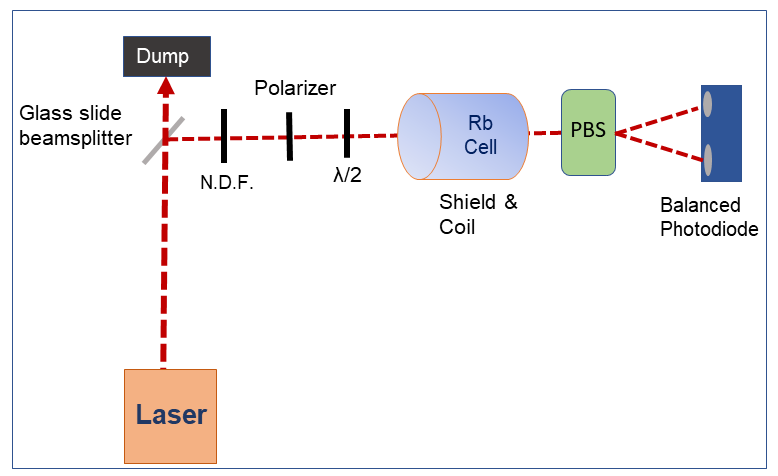
\includegraphics[width=0.8\textwidth]{figures/experimental_setup_zero_field}
\caption{Schematic diagram of experimental setup for zero field NMOR measurement (discussed in the text).\label{fig:zerofield}.}
\end{figure}

Fig.\ref{fig:zerofield} schematically depicts a top view of the Rb
magnetometer, as it may be used for measurements of the magnetic field
within a few hundred pT of zero.  This mode was used, for example, in
Ref.~\cite{bib:nmor} to measure the axial magnetic shielding factor of
the passive magnetic shielding system.  In this thesis, this operation
mode was not normally used because we desired to develop the system
for larger magnetic fields.  But it is nonetheless instructive to
demonstrate the starting point of my thesis research.  We also used
this mode to study our process of degaussing of the magnetic shields,
which was also being developed.

An external cavity diode laser produces light near the Rb D1
transition.  The laser is tuned near the $^{85}$Rb $F=3,2\rightarrow
2$ absorption minimum.  A microscope slide is used as a beamsplitter
in order to divert a reduced power into the experiment.  The power is
further reduced using neutral density filters (indicated by N.D.F. in
Fig.~\ref{fig:zerofield}).  A linear polarizing sheet is oriented at a
45$^\circ$ angle relative to the vertical direction.  Since the laser
beam is polarized, this further reduces the power by a factor of
two. The laser power after this point is normally in the range of
2-20~$\mu$W.  Small adjustments to the incident plane of polarization
may be made by a $\lambda/2$ plate.

The beam then passes through a paraffin-coated cell containing Rb
vapour.  The cell is within a magnetic shielding and field generation
system that produces a uniform field along the beam axis.  The plane
of polarization of the laser light will rotate slightly as it passes
through the cell because of non-linear magneto-optical effects.  A
balanced polarimeter is used to analyze the optical rotation of the
laser light resulting from the interaction of the laser light with the
atoms in the cell.  The polarimeter consists of a polarizing beam
splitter (a Wollaston prism) which splits the beam into its vertical
and horizontal polarization components.  Each component is sensed by a
balanced photodiode which outputs the difference in light intensities.
If the polarizer is set at a 45$^\circ$ angle and aligned with the
axis of the $\lambda/2$-plate, and in the absence of any optical
rotation, the balanced photodiode would output zero volts.  If the
plane of polarization is rotated by passage through the cell, it will
be sensed by the differential photodiode signal.  This is discussed
further in Section~\ref{sec:Signal Processing}.

Results of the operation of the zero-field magnetometer are discussed
further in Sections~\ref{sec:something-in-ch4}
and~\ref{sec:degaussing-section-in-ch5}.  In order to measure fields
farther from zero, a pump-probe technique is used, where the amplitude
of the pump beam is modulated.

\begin{figure}%[h]
\centering
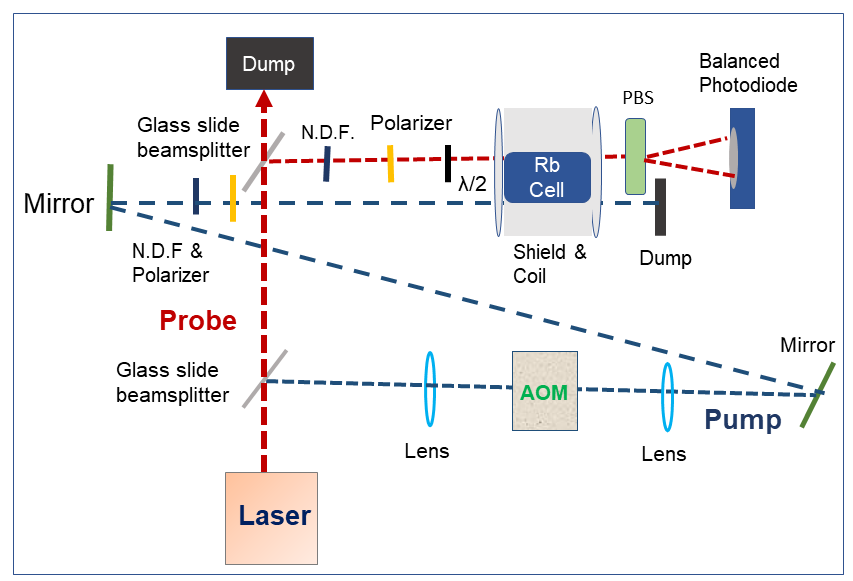
\includegraphics[width=0.95\linewidth]{figures/experimental_setup}
\caption{Schematic diagram of the experimental setup for measuring
  rotation of the polarization plane with amplitude modulated (AM)
  light. AOM stands for acousto optic modulator, $\lambda/2$ - half
  wave plate, N.D.F- neutral density filter, PBS- polarizing beam
  splitter.\label{fig:pumpprobe}}
\end{figure}

Fig.~\ref{fig:pumpprobe} shows the schematic layout of the apparatus
used for studying the non-linear magneto-optical effects with the
amplitude modulated light. This experimental setup is used in Forced
oscillation scan and FID NMOR discussed in
Section~\ref{sec:Forced-Oscillation Mode} and~\ref{sec:FID}.

% I think you said all this already, or can leave it for the more
% detailed systems which follow.

%In this work, a paraffin-coated vapor cell (about 5~cm long)
%containing natural rubidium with stable isotopes $^{87}$Rb and
%$^{85}$Rb, is used as the magneto-optical sample. A semiconductor
%diode laser is the light source. The laser wavelength
%($\lambda=795$~nm) is precisely controlled by an external locking
%system.

Pump and probe beams are created from the main beam using microscope
slides as beam splitters. The typical light power of the pump beam is
40 $\mu$W (time-averaged) and the typical light power of the probe
beam is 20 $\mu$W.  An acousto-optic modulator (AOM) is used to
modulate the amplitude of the pump beam, normally as a square wave
with low duty cycle.  The details of the working principle of AOM is
discussed in Section~\ref{sec:AOM}.  The pump beam is focused into the
AOM and re-parallelized afterward using two lenses of the same focal
length.  Before interact with the Rb cell pump beam then passes
through an N.D.F to adjust the beam power, and then a linear
polarizer.  After that the linearly polarized light beam interacts with
Rb atoms.

The probe beam follows essentially the same path as for the zero-field
magnetometer.  The nonlinear Faraday rotation signals are analyzed by
a balanced polarimeter.  A Wollaston prism (labelled as PBS in
Fig.~\ref{fig:pumpprobe}) is used to split the beam into its
perpendicular polarization axes which are then analyzed individually
by a differential photodiode.

\begin{table}%[h]
\centering
\begin{tabular}{|l|c|}\hline
\textbf{ Position}    & \textbf{Laser Power($\mu$W)} \\ \hline
AOM &4000  \\
Pump beam (time averaged) & 60  \\
Probe beam & 22  \\
After Cell & 18   \\\hline
\end{tabular}
\caption{Adjusted laser power at several positions in the
  experiment.\label{table:laser power}}
\end{table}

In this case, the optical rotation is also modulated near the pump
modulation frequency.  A lock-in amplifier is used to demodulate the
signal. Table~\ref{table:laser power} shows the typical beam power at
several positions in the experimental setup.



\section{External Cavity Diode Laser}

In our NMOR based optical magnetometry setup, laser light is provided
by an external cavity diode laser (ECDL).  
%These kind of diodes are
%semiconductor diodes and thus vibration and shock resistant.
%They are
%also wavelength tunable.
ECDLs emit a single mode laser light with a very narrow linewidth
($\sim 100$~kHz).
%A critical aspect of an ECDL is temperature control
%of the cavity, since the laser frequency depends on the cavity length
%and hence on the thermal expansion coefficient of the cavity
%material. Micrometer screws enable manual coarse tuning, while precise
%scans without mode hops are performed by a piezo actuator. This kind
%of grating stabilized diode lasers is especially advantageous for
%spectroscopy with the alkalines.
Our Toptica DL-100 outputs a tunable wavelength near 795 nm with an
output power $<100$ mW. The laser spot size is elliptical, and
approximately 3 mm x 5 mm = $15 mm^2$.  The laser was typically tuned
to the D1 ($F=3,2\rightarrow 2$) absorption minimum.  This was done
using the feed-forward function of the ECDL, where the laser current
and external cavity length are swept simultaneously to prevent mode
hopping.  The final tuning was then adjusted to maximize the optical
rotation signal.

\section{Dichroic Atomic Vapor Laser Lock (DAVLL)}

In order to control the laser frequency to a fraction of the
Doppler-broadened linewidth of the relevant hyperfine atomic
transition of the Rb D1-line, a frequency error signal is generated by
taking usage of the Zeeman effect combined with circular dichroism of
an atomic vapor which is exposed to a magnetic
field~\cite{doi:10.1063/1.3568824}. The generated error signal passes
through zero crossings as the laser frequency coincident with the lock
frequency.  A feature of optics setup of
Ref.~\cite{doi:10.1063/1.3568824} is that the lock point can be
adjusted by physically rotating optical elements to achieve the desire
zero-crossing.
\begin{figure}%[h]
\centering
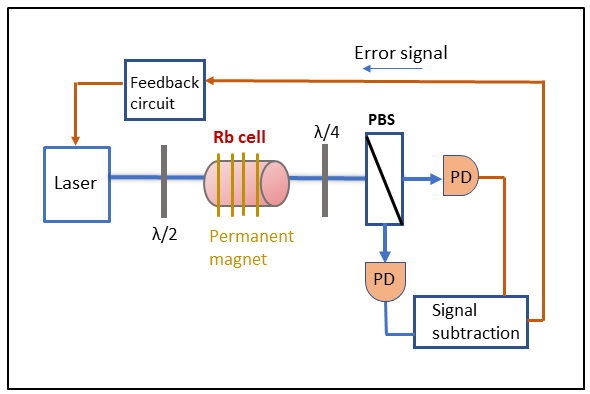
\includegraphics[width=0.8\linewidth]{figures/DAVLL}
\caption{Schematic diagram of experimental setup for characterizing the DAVLL. PBS- polarizing beam splitter, PD- photodiode.\label{fig:DAVLL}}
\end{figure}
The schematic diagram of the apparatus used in the DAVLL system has
shown in Fig \ref{fig:DAVLL}. Linearly polarized laser light is
incident on a glass cell filled with Rb vapor surrounded by a set of
permanent magnets. In this magnet arrangement a layer of ceramic
magnets and a layer of flexible magnetic stripping are placed one
after another and a customized holder is used to hold the pieces
together.  A picture of the magnets and cell is shown in
Fig.~\ref{fig:magnet}.
%Then the magnet holder is placed on the tp of Newport 271 Lab Jack
%which is uniquely designed to provide smooth, stable height
%adjustment and high load capacity.
The wave vector of the light is parallel to the axis of the generated
magnetic field by the permanent magnets. After the interaction of the
laser beam with the Rb cell, the beam passes through a quarter-wave
plate before impinging on a polarizing beam splitter (PBS).  In our
experiments we used a polarizing cube beamsplitter. The linearly
polarized beam incident can be split into two orthogonal circularly
polarized beams by this arrangement. A set of photodiodes are used to
detect the intensity of the right and left circularly polarized
beams. Both of the photodiodes are attached to a polarimeter board
which is used to measure the difference in signals and amplifies it. A
Tektronix TDS2024 oscilloscope is used for monitoring each photodiode
signal as well as the difference output. The signal is then fed into a
PID controller which finally controls the laser diode current
corresponding to a certain laser frequency.

\begin{figure}%[h]
\centering
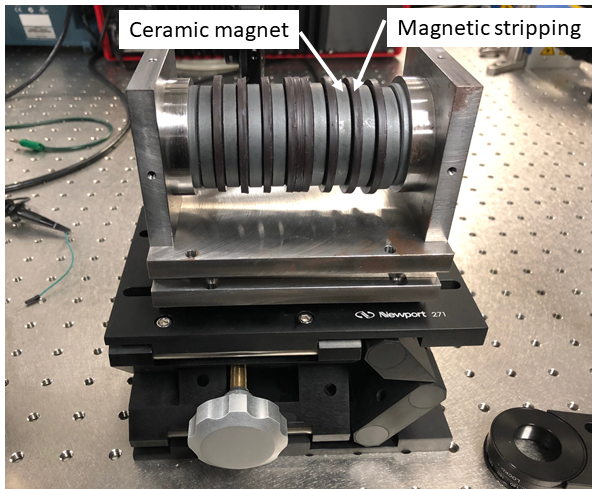
\includegraphics[width=0.7\linewidth]{figures/magnet.png}
\caption{Picture of cell-magnet arrangement in the DAVLL system.\label{fig:magnet}}
\end{figure}

\section{Laser tuning and locking}


\begin{figure}%[h]
\centering
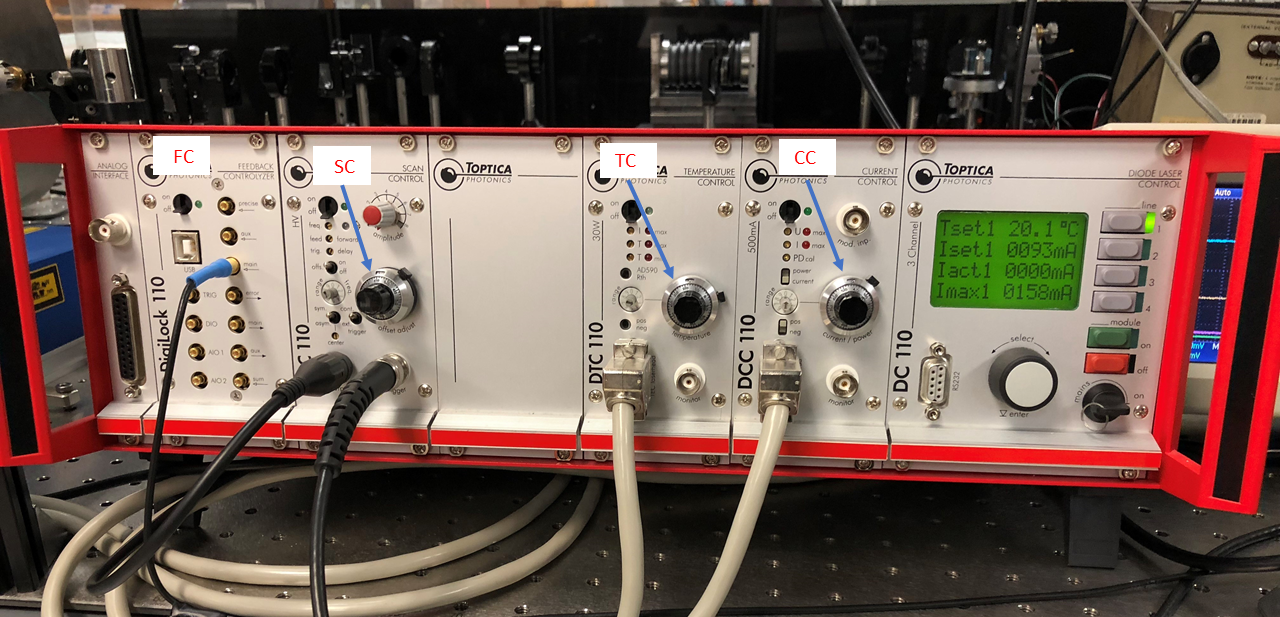
\includegraphics[width=\linewidth]{figures/laser_control_}
\caption{Diode laser controller unit consist of analog current control
  module (CC), scan control module (SC), temperature control module
  (TC), feedback controlyzer (FC) and Diode Laser Controller
  display.\label{fig:laser controller}}
\end{figure}


In order to polarize atoms by optical pumping, it's important to tune
the laser properly to expected transition line.  A photograph of the
laser power supply and control system is shown in
Fig.~\ref{fig:laser-controller}.  The diode temperature selects the
desired power at the wavelength of interest, and was typically set to
20.1$\degree$C.  The laser current is then adjusted to select the mode
of the diode near the Rb D1 line.  By adjusting the laser current and
piezo-electric cavity length control, a mode-hop free region was
selected for tuning.  Tuning to the transition of interest was then
done using ``offset adjust'' knob of the scan control system, which
controls the feed-forward system described earlier, adjusting both the
laser current and piezo voltage simultaneously with a fixed constant
of proportionality between them.

\begin{figure}%[h]
\centering
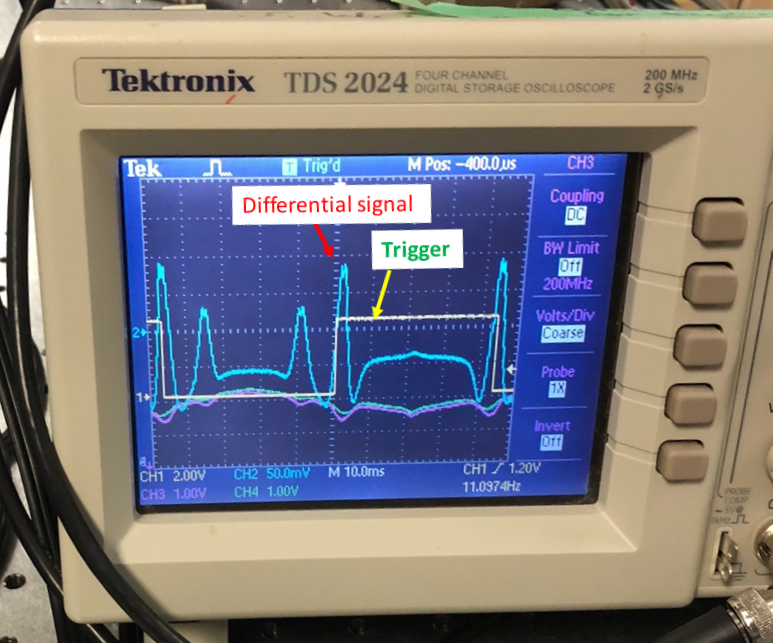
\includegraphics[width=0.85\linewidth]{figures/laser-tune.png}
\caption{Oscilloscope trace of DAVLL signals during
  tuning.\label{fig:laser-tune}}
\end{figure}

Tuning is usually done while the feed-forward is scanning, by
adjusting the offset adjust while looking at the signals in the DAVLL
system.  An oscilloscope is used to observe the output of each PD and
the differential amplifier of the DAVLL system.  The scope is
triggered by the trigger output on the scan control (SC) panel.  Laser
current can be controlled by adjusting the current control knob until
the spectral structure of $^{85}$Rb appears (see
Fig.~\ref{fig:laser-tune}). we need to keep adjusting the current
control knob until a maximum symmetry between the upsweep and
downsweep portions is achieved. After that by adjusting the
``amplitude'' knob of the SC panel we can zoom in the structure and
tune the central frequency of the scan to the absorption minima.

\begin{figure}%[h]
\centering
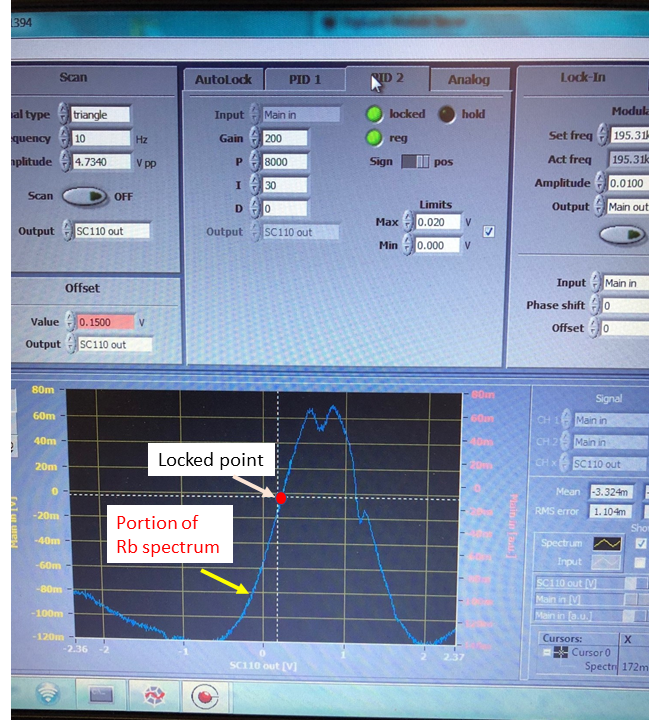
\includegraphics[width=0.7\linewidth]{figures/digilock.png}
\caption{Digilock graphical user interface.\label{fig:digilock}}
\end{figure}

The Digilock 110 feedback controlyzer (FC) is used for laser locking,
using a PID system.  It offers graphical user interface shown in
Fig.~\ref{fig:digilock}.  The FC is connected by USB to a computer
where Digilock software is installed. The output signal of the
differential photodiode is fed into the FC main input.  After
connecting the DigiLock 110 I turn on its scan function and navigate
to the autolock screen at the bottom. Then the the portion of the
spectrum that I tuned earlier will appear (see
Fig.~\ref{fig:digilock}). Then I select the crosshairs tool which
allow us to drag the crosshairs on the part of the spectrum that we
want to tune to. Finally for successful laser locking we need to click
and select ``PID lock to slope'', selecting the exact lock point on
the computer screen.  PID parameters were adjusted to give a
relatively low-bandwidth lock.  For most of the studies reported in
this thesis we use the auto locking features of the DigiLock software.


\section{Acousto-optic Modulator (AOM)\label{sec:AOM}}

The acousto-optic modulator (AOM) offers a method of modulating the
amplitude of the laser light.  The AOM is used to modulate the
amplitude of the pump beam. The pump beam is linearly polarized light,
and so the amplitude is modulated at $2\omega_L$.  For 1~$\mu$T field
the AOM operation frequency is 9335 Hz and the AOM driving frequency
is 2034 Hz when the magnetometer operate at $0.2~\mu$T.  This form of
pumping generates a coherent precession of an axis of alignment in the
atoms in the Rb cell. In FID mode, once the coherence has been
sufficiently established, the AOM may be switched off in order to
measure the precession frequency of the state using the probe beam.

\begin{figure}%[h]
\centering
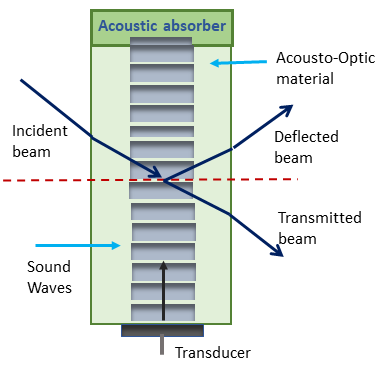
\includegraphics[width=0.7\linewidth]{figures/AOM}
\caption{Principle of an acousto-optic modulator.\label{fig:aom}}
\end{figure}

The principle of operation of an AOM is shown in Fig.~\ref{fig:aom}.
The AOM contains a crystal which has a piezoelectric transducer
attached at the end that propagates acoustic waves within the medium.
An RF signal is applied to the transducer to generate the acoustic
wave. The compression and refraction of the sound waves result in
periodic variations of the refractive index of the medium which form a
diffraction grating.  Incident laser light will be diffracted by the
grating, generally providing a number of diffracted beams. The
strength of the sound wave is directly related to the intensity of the
defracted light. Depending on the interaction length $L$, laser
wavelength $\lambda$ in the medium and the sound wavelength $\Lambda$
it is possible to operate AOM in two different modes, the Raman-Nath
regime and the Bragg regime. For our experiment we operated in the
Bragg regime.

In the Bragg regime~($L>\Lambda^2/\lambda$) the light beam enters
the medium at one particular Bragg angle
\begin{equation}
\theta_B=\frac{\lambda}{2\Lambda}.
\end{equation}                                 
The observed diffraction pattern generally consists of two diffraction
maxima; these are the zeroth and the first orders. In this case the
possible maximum intensity of the first order diffracted light can be
near 100\%.  Generally in our setup we generally achieve $\sim 10$\%.
Due to this relatively high efficiency, the first order light can be
used for amplitude modulation.

For this experimental setup, an Isomet 1205C-1 AOM is used with an RF
center frequency of 80 MHz. The AOM uses a crystal of lead molybdate
(PbMoO$_4$) for the optical interaction medium and lithium niobate as
the piezoelectric transducer.  The amplitude modulating pulses are
driven with an Isomet 532C-2 AO driver with video input range 0.0 V to
1.0 V.  An Agilent 33522A function generator is used to regulate the
AOM driver.

This amplitude modulation in our experiments was generally done by a
square wave modulation with a duty cycle of 1-10\%. For this specific
model of AOM driver the RF rise/fall time is smaller than 6 nsec. The
active aperture of the modulator is tiny (1~mm) and light is focused
into the AOM and recollimated afterward.  In order to reach maximum
deflected light intensity small adjustments are made near the Bragg
angle.


\section{Rb Cell}

When glass cell is used to store alkali atoms, the atomic mean free
paths increase and alkali spins depolarize immediately after making
non-elastic collision with the glass walls. Prolonging the atomic
alignment is crucial to achieving ultra-narrow NMOR resonance
widths. So it is necessary to prevent depolarizing collisions to
achieve the longer lifetimes of atomic ground state
coherences~\cite{PhysRevA.72.023401,Balabas:10,doi:10.1063/1.3236649}.
This can be achieved by coating the inner walls of the cell with
anti-relaxation materials, in our case paraffin.  Paraffin can
preserve the polarization of the atoms after $\sim 1000$ wall bounces
before depolarizing~\cite{PhysRev.147.41,PhysRevA.72.023401}.

\begin{figure}%[h]
\centering
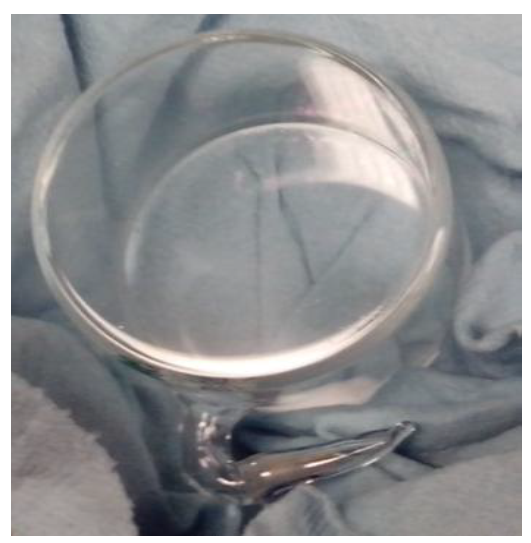
\includegraphics[width=0.5\linewidth]{figures/cell}
\caption{Paraffin coated Rb cell.\label{fig:rb-cell}}
\end{figure}

A photograph of the paraffin-coated vapour cell used in this work is
shown in Fig.~\ref{fig:rb-cell}.  The cell contains natural rubidium
with stable isotopes $^{85}$Rb and $^{87}$Rb.  The cell is
cylindrical, 5~cm long and 5~cm in diameter with optical flats on the
ends.  The cell was provided by D.~Budker, having been prepared in a
fashion similar to the cells described in
Ref.~\cite{PhysRevA.72.023401}.  For Ref.~\ref{bib:nmor-shielding},
our group characterized the cell using a method similar to
Ref. \cite{PhysRevA.72.023401}, by measuring the relaxation of
longitudinal polarization using optical rotation as a probe.  The long
time component of the relaxation was thereby found to decay with a
time scale of 400~ms.  Longer relaxation time indicates good quality
of cell.  It was also characterized magnetometrically using the
zero-field mode of operation and found to have a width near zero field
competitive with the typical 2~$\mu$G widths achieved by
Budker~\cite{bib:budkers-phys-rev-1998-paper}.  The temperature of the
vapour cell was controlled by the ambient temperature of the
surrounding room ($\sim 21\degree$).  Although the temperature can be
increased closer to the Rb melting point, we did not try this in the
present work.  In future work we plan to use Cs vapour cells which
naturally have a higher vapour pressure.

\section{Magnetic field system}

The magnetic field system consists of a four-layer $\mu$-metal
magnetic shielding, degaussing system and internal coils.

\subsection{Magnetic Shielding}

\begin{figure}%[h]
\centering
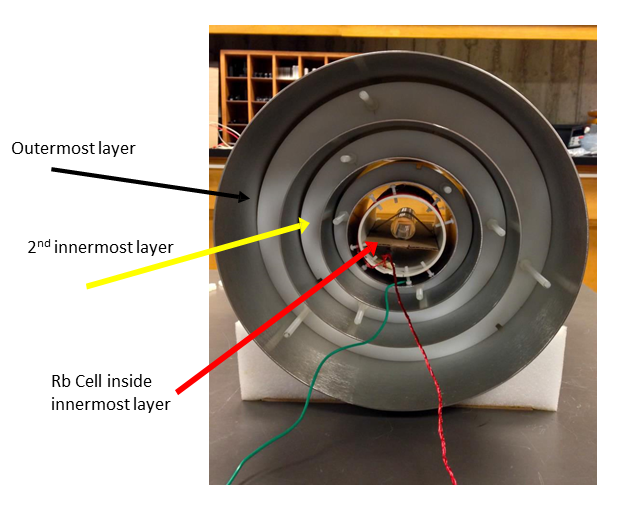
\includegraphics[width=0.8\linewidth]{figures/magnetic_shielding}
\caption{Four layer $\mu$-metal magnetic shielding. The diameter of
  each endcap is larger by 0.1 cm to fit over its corresponding
  cylinder. The hole diameter and stovepipe length for each endcap are
  the same. High density polyethylene spacers and nylon thread
  rods/nuts are used to hold the shields and end caps
  together.\label{fig:shield-picture}}
\end{figure}

In precision magnetometry, magnetic shielding is required to achieve
well characterized, stable magnetic field conditions independent of
the Earth’s magnetic fields and environmental perturbations.  A
picture of the magnetic shield and internal coil system is shown in
Fig.~\ref{fig:shield-picture}.  Then endcaps of the shield have been
removed for clarity.  The white cylinder within the shield is where
the former upon which the internal coil has been wound.  The
photograph shows a different (lower quality) paraffin-coated cell than
used in this work.

\begin{figure}%[h]
\centering
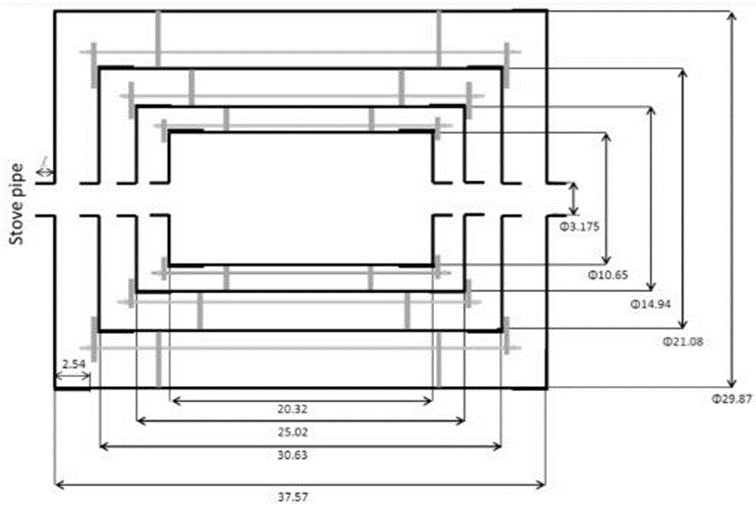
\includegraphics[width=0.8\linewidth]{figures/shield.JPG}
\caption{Schematic diagram of the 4-layer magnetic shield (dimensions
  in cm).\label{fig:shield}}
\end{figure}

Fig.~\ref{fig:shield} shows a schematic diagram indicating the
measurements of the magnetic shield system.  The design process for
the shield is discussed in Ref.~\cite{bib:nmor}.  The axial magnetic
shielding factor was measured using the zero-field magnetometer in
Ref.~\cite{bib:nmor} and found to be $10^7$, which is consistent with
a relative magnetic permeability of $\mu_r=20,000$ for the material
used in the shielding layers.  All access (for laser light and wires
for coils) is made through holes in the endcaps.  The innermost
magnetic shielding layer is 4'' in diameter and 8'' long, limiting the
space available for experimental equipment.

% Shielding
%ratio T is a parameter to evaluate the efficiency of a shield which
%can be expressed as
%\begin{equation}
% T = \frac{B_{in} }{B_0} 
%\end{equation}
%where $B_0$ is the homogeneous magnetic field in free space, and $B_{in}$ is the field induced in the presence of shield due to  $B_0$. Using multi-layer shielding is an efficient way to enhance shielding efficiency \cite{doe:website2} . The effectiveness of a multilayer shield with thin shells having wide gaps between them is same as the much heavier and more expensive thick, single layer shield.
%The optimization of the air gaps between the shells is important to minimize the total size of a multilayer shield. When a coil is placed inside the innermost layer of passive shield the shield turns into a return yoke. As a result, the magnitude of field $B_0$ increase. A four layer $\mu$-metal magnetic shielding with nearly spherical geometry is used for this highly sensitive Rb magnetometer. $\mu$-metal is a very high permeability nickel based alloy, which is used for shielding low-frequency magnetic field. When the shape is close to a sphere we will get zero magnetic field inside independent of the outside field.

%The inner radius of the innermost shield is 18.44 cm, equal to its half-length. The radii and half-lengths of the progressively larger outer shields increase geometrically by a factor of 1.27.  Each cylinder has two endcaps which possess a 7.5 cm diameter central hole \cite{Andalib:2016ahj}. A stove-pipe of length 5.5 cm is placed on each hole was designed to minimize leakage of external fields into the progressively shielded inner volumes. The magnetic shielding factors of each of the four cylindrical shells, and of various combinations of them, were measured and found to be consistent with $\mu_r \sim 20, 000$ \cite{Martin:2014foa}


\subsection{Degaussing system\label{sec:Degaussing}}

Our four layer $\mu$ metal magnetic shield is designed to minimize the
magnetic field at the cell, but magnetic hysteresis limits the
magnetic field in any region to be exactly zero. Degaussing
(demagnetizing) process is used to reduce the background magnetic
field inside the shield. Although Rb cell is securely placed inside
the four layer mu-metal shielding it is necessary to demagnetize the
shield before every measurement session to eliminate accidentally
created local magnetizations.

\begin{figure}%[h]
\centering
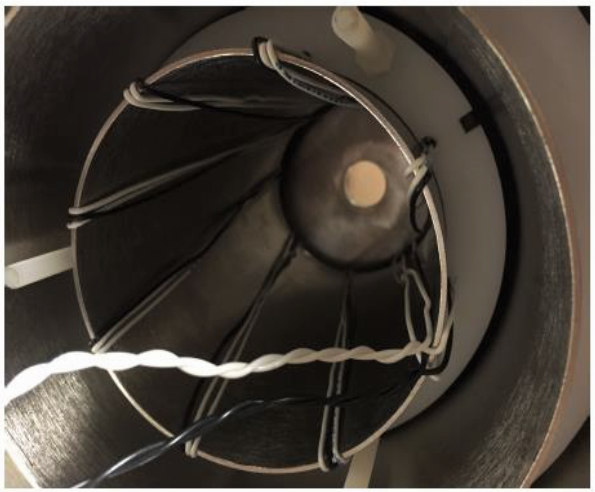
\includegraphics[width=0.6\linewidth]{figures/degaussing_coil.png}
\caption{Photograph of degaussing coil.\label{fig:degaussing_ccoil.}}
\end{figure}

 For degaussing a special coil (like the 16 turn white wire  shown in Fig \ref{fig:degaussing_ccoil.}) is wind around inner most layer of shielding  in toroidal configuration
and  since the endcap of innermost shield is open it might important to degauss the outer layers of shield. Toward this end, a single turn wire is wind around the outer 3-layers of shielding.
In practice, demagnetizing is achieved  by supplying the coil with oscillating current. The current amplitude decreases depending on the chosen envelope function starting from a current that yields magnetic saturation inside the ferromagnetic material, down to zero. 
\begin{figure}[h]
\centering
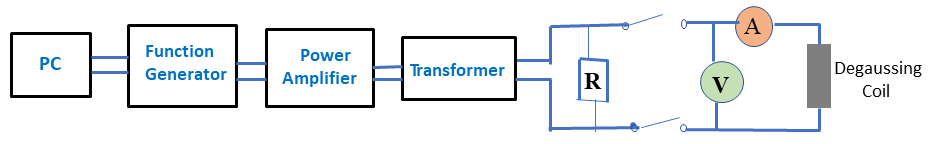
\includegraphics[width=1.0\linewidth]{figures/degaussing_system}
\caption{Schematic diagram of degaussing system consist of function generator, power amplifier, transformer, variable resistor(R), 1 $\ohm$ sense resistor (A), oscilloscope (V) and degaussing coil. \label{fig:schematic-of-degaussing_system.}}
\end{figure}

In our degaussing system, an Agilent 3522A function generator  provides a ramped sinusoidal that controls a current supply driving the degaussing coil \cite{Martin:2014foa}. The wires going to the degaussing loop should be twisted together to avoid picking up or causing noise.  A DCP 260 Servowatt is used as the amplifier for degaussing system which outputs $\pm$ 60~V at idle and nominal output current is  $\pm$ 5 A. The used transformer for this setup is a  HS1B250 hevi-duty transformer which provide unity gain (wire connection is set to in 240:240 mode). The frequency of the transformer is  60 Hz.  A double-pole, double-throw (DPDT) switch is used to electrically connect and disconnect the degaussing coil from the circuit. The function generator settings has discussed in Table \ref{table:degaussing setting}. For our degaussing system we are using an envelope function which has $1\times 10^6$ points. Degaussing is complete after $5\times 10^6$ points. Sample rate affects how quickly we move through this waveform. If sample rate is set to 10000 samples/sec and the frequency of the carrier wave is set to 10 Hz then it means 500 cycles were completed. 
 \begin{table}%[h]
\centering
\begin{tabular}{|l|l|}
\hline
\textbf{ SETTING}    & \textbf{ VALUE} \\
\hline
Function generator &   \\
\hline
Frequency &  10 Hz   \\
Sample rate    &  10000 sample/sec  \\
Amplitude   &   10 V \\
Offset  &       0 V  \\
\hline
\end{tabular}
\caption{Setting for degaussing system \label{table:degaussing setting}}
\end{table}


\subsection{Internal coil\label{sec:Internal coil}}
 For the Rb atomic magnetometer an internal coil referred as z-coil is used to provide the magnetic field along the axis of light propagation direction (z-direction). This coil produces uniform field in the ROI  of magnetic shielding. The z-coil was wound on a 7.62 cm diameter, 20.32 cm long ABS plastic pipe. Seven turns of 26 AWG magnet wire were wound at 2.54 cm spacing, with 1.27 cm spacing from the magnetic faces of the endcaps of the innermost magnetic shield. The spacings were chosen so that, in the infinite permeability limit, and in the limit where the axial aperture holes in the endcaps are small, the boundary conditions would produce image currents forming an infinitely long solenoid. Two saddle coils were wound on the same cylinder in order to control transverse fields( along x and y direction) internally; these were normally disconnected during precision measurements. The internal coil system was calibrated using a three-axis fluxgate magnetometer at fields of ∼100 nT.  The calibration constant for z coil is 48 nT/mA and the calibration constant for x and y coil is 25 nT/mA. The calibration of the z-coil was verified using the NMOR magnetometer with an AM pump beam, and the known gyromagnetic ratios of~ $^{85}Rb$ and $^{87}Rb$. Homogeneity of the residual field and magnetic field generated by the coil system was measured by scanning a fluxgate magnetometer along the axis of the system with and without the coil energized. At a field of 1 $\mu$T, the axial field generated by the coil was uniform within the ROI to the $1\%$  level.


\section{Lock in Amplifier}
SR830 DSP Lock in Amplifier is a elementary part in the DAQ system of Rb magnetometry. It can measure very  small voltages. The most attractive feature of a lock in amplifier is that it is able to suppress all noise contributions which differ from the reference frequency. A reference signal is applied to the lock-in amplifier which is usually done by an external oscillator which passes a discriminator. In this magnetometry setup sync output of a function generator is used as external reference signal for force oscillation scan. The external reference signal is phase locked to an internal reference frequency, provided internal oscillator of the lock-in.Since a lock-in amplifier has two phase sensitive detectors we obtain two output signals. During the process of phase sensitive detection (PSD), the reference signal is first multiplied with the real input signal  and in a second stage, the real input signal is multiplied by
the lock-in reference signal with a phase shift of $90\degree$. Then a lowpass filter is used to filter both signals. The first one is referred to as X output and the 2nd output signal is referred to as Y output. X output is knows as in phase component and the Y output is called out of phase component.


\section{Signal Processing\label{sec:Signal Processing}}
Sensitive magnetometry requires detection of extremely small optical rotation angles. There are numerous methods for detecting the optical rotation of the probe beam.  we instead use the balanced polarimetry technique.  Transmitted light was analyzed for optical rotation by a balanced polarimeter system containing a Wollaston prism and a Newport model 2307 balanced photo receiver. The power delivered to the vapour cell was typically 15 $\mu$W, measured periodically using a Newport model 818-SL power meter inserted into the
beamline. After the cell the probe beam passes through a polarizing beamsplitter set at 45\degree~to the initial polarization direction resulting in two separate beams with individual intensities given by 
\begin{equation}
I_1 = I_0\sin^2(\theta-\frac{\pi}{4})
\end{equation}

\begin{equation}
I_2 = I_0 \cos^2(\theta-\frac{\pi}{4})   
\end{equation}

such that $I_1 + I_2 = I_0$, and the intensities are balanced when $\theta = 0$ and unbalanced otherwise. 
For small rotations $\theta << 1$ in terms of power we can write,
\begin{equation}
  \theta \approx \frac{P_1-P_2}{2(P_1-P_2)}  
\end{equation}

where $P_1$ and $P_2$ represent signals of the two photodiodes in the polarimeter. The differential value is acquired with a lock-in amplifier (LIA) referenced to the pump beam modulation provided by a function generator. The demodulated signal from the LIA is acquired by a personal computer for analysis. 

